\documentclass[aspectratio=169]{beamer}

% ---------- ENCODING & FONTS ----------
\usepackage[utf8]{inputenc}
\usepackage[T1]{fontenc}

% ---------- THEME & LOOK ----------
\usetheme{Madrid}
\usecolortheme{seahorse}
\usefonttheme{professionalfonts}
\setbeamertemplate{navigation symbols}{}
\setbeamercovered{transparent}
\setbeamertemplate{itemize items}[circle]
\setbeamertemplate{enumerate items}[default]
\setlength{\parskip}{0.25em}

% ---------- COLORS ----------
\definecolor{accent}{RGB}{0,92,184}
\definecolor{soft}{RGB}{233,244,255}
\definecolor{canadared}{RGB}{196,30,58}
\definecolor{leafgreen}{RGB}{0,130,80}
\definecolor{goldenrod}{RGB}{218,165,32}
\definecolor{deeporange}{RGB}{220,90,20}
\definecolor{shiftpurple}{RGB}{130,50,180}
\definecolor{tealblue}{RGB}{0,128,128}
\definecolor{lightred}{RGB}{245,210,210}
\setbeamercolor{structure}{fg=accent}
\setbeamercolor{title}{fg=white,bg=accent}
\setbeamercolor{frametitle}{fg=accent}
\setbeamercolor{block title}{bg=accent!12,fg=accent}
\setbeamercolor{block body}{bg=soft}

% ---------- PACKAGES ----------
\usepackage{booktabs}
\usepackage{amsmath, amssymb}
\usepackage{array}
\usepackage{multirow}
\usepackage{hyperref}
\usepackage{tikz}
\usepackage{pgfplots}
\pgfplotsset{compat=1.18}
\usetikzlibrary{arrows.meta, positioning, calc, shapes.geometric}
\hypersetup{colorlinks=true,linkcolor=accent,urlcolor=accent}

% ---------- SAFE TRANSITION FALLBACK ----------
\makeatletter
\@ifundefined{transfade}{\newcommand{\transfade}[1][]{}}{}
\makeatother

% ---------- TITLE ----------
\title{\textbf{Unemployment and Inflation}}
\subtitle{{\large ECON 101 -- Principles of Macroeconomics}}
\author{Muhebullah Karimzada}
\date{Spring 2026}

% ============================================================
\begin{document}
% ============================================================

\begin{frame}[plain]
  \titlepage
\end{frame}

\begin{frame}{Chapter Outline}
\transfade
\begin{itemize}[<+->]
  \item \textbf{5.1} Measuring the Unemployment Rate and the Labour Force Participation Rate
  \item \textbf{5.2} Types of Unemployment
  \item \textbf{5.3} Explaining Unemployment
  \item \textbf{5.4} Measuring Inflation
  \item \textbf{5.5} Using Price Indexes to Adjust for the Effects of Inflation
  \item \textbf{5.6} Real versus Nominal Interest Rates
  \item \textbf{5.7} Does Inflation Impose Costs on the Economy?
\end{itemize}
\end{frame}

\begin{frame}{Why Unemployment and Inflation Matter}
\transfade
\begin{itemize}[<+->]
  \item Previous chapter: how to measure \textbf{total output} (GDP).
  \item This chapter: how to measure
  \begin{itemize}[<+->]
    \item \textbf{Unemployment} in the labour market, and
    \item \textbf{Inflation} in the goods and services market.
  \end{itemize}
  \item \textbf{Canadian context:} In 2024, the unemployment rate averaged $\approx$6.3\% and CPI inflation was $\approx$2.7\% --- both central targets of Bank of Canada policy (Bank of Canada MPR, 2024).
\end{itemize}
\end{frame}

% ============================================================
\section{5.1 Measuring Unemployment and Labour Force Participation}
% ============================================================

\begin{frame}{5.1 Learning Objective}
\transfade
\begin{block}{Goal}
Understand how unemployment, labour force participation, and employment rates are measured.
\end{block}
\begin{itemize}[<+->]
  \item Canada has $\approx$32 million working-age people --- we cannot track everyone individually.
  \item Statistics Canada uses the \textbf{Labour Force Survey (LFS)}: $\approx$56,000 households sampled monthly.
  \item Each working-age person (15+) is classified as \textbf{employed}, \textbf{unemployed}, or \textbf{not in the labour force}.
\end{itemize}
\end{frame}

%--- Fig 5.1: LFS classification flow diagram ---
\begin{frame}{Figure 5.1 -- Employment Status: How the LFS Classifies Canadians}
\begin{center}
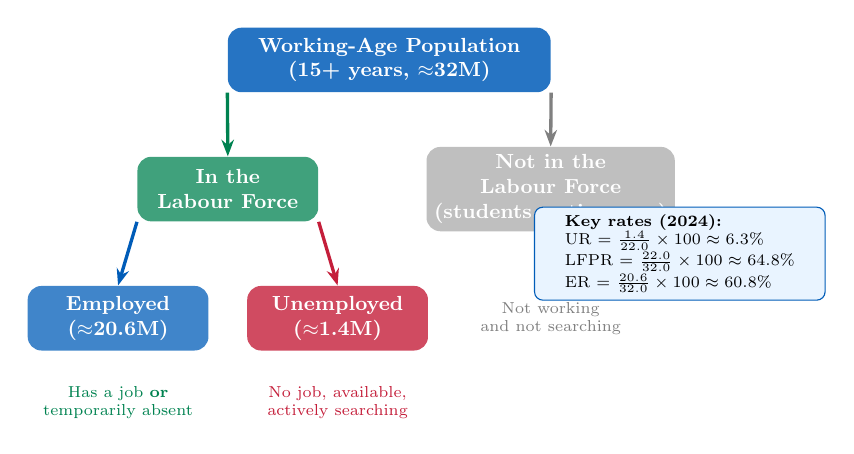
\begin{tikzpicture}[
  box/.style={rectangle, rounded corners=5pt, align=center,
              font=\small\bfseries, minimum width=2.8cm, minimum height=1cm},
  scale=0.82, transform shape
]
  % Working-age population
  \node[box, fill=accent!85, text=white, minimum width=5cm] (wap)
    at (0,3.5) {Working-Age Population\\(15+ years, $\approx$32M)};

  % Labour force
  \node[box, fill=leafgreen!75, text=white] (lf)
    at (-2.5,1.5) {In the\\Labour Force};
  % Not in LF
  \node[box, fill=gray!50, text=white] (nilf)
    at (2.5,1.5) {Not in the\\Labour Force\\(students, retirees\ldots)};

  % Employed / Unemployed
  \node[box, fill=accent!75, text=white] (emp)
    at (-4.2,-0.5) {Employed\\($\approx$20.6M)};
  \node[box, fill=canadared!80, text=white] (unemp)
    at (-0.8,-0.5) {Unemployed\\($\approx$1.4M)};

  % Arrows
  \draw[-{Stealth[length=6pt]}, very thick, color=leafgreen]
    (wap.south west) -- (lf.north);
  \draw[-{Stealth[length=6pt]}, very thick, color=gray]
    (wap.south east) -- (nilf.north);
  \draw[-{Stealth[length=6pt]}, very thick, color=accent]
    (lf.south west) -- (emp.north);
  \draw[-{Stealth[length=6pt]}, very thick, color=canadared]
    (lf.south east) -- (unemp.north);

  % Formulas below
  \node[font=\scriptsize, align=center, text=leafgreen]
    at (-4.2,-1.8) {Has a job \textbf{or}\\temporarily absent};
  \node[font=\scriptsize, align=center, text=canadared]
    at (-0.8,-1.8) {No job, available,\\actively searching};
  \node[font=\scriptsize, align=center, text=gray]
    at (2.5,-0.5) {Not working\\and not searching};

  % Key rates
  \node[draw=accent, rounded corners=3pt, fill=soft, font=\scriptsize, align=left,
        minimum width=4.5cm] at (4.5,0.5)
    {\textbf{Key rates (2024):}\\
     UR = $\frac{1.4}{22.0}\times100\approx6.3\%$\\
     LFPR = $\frac{22.0}{32.0}\times100\approx64.8\%$\\
     ER = $\frac{20.6}{32.0}\times100\approx60.8\%$};
\end{tikzpicture}
\end{center}
\end{frame}

\begin{frame}{Key Labour Market Rates}
\transfade
\begin{itemize}[<+->]
  \item \textbf{Unemployment rate (UR):}
  \[
    \text{UR} = \frac{\text{Number unemployed}}{\text{Labour force}} \times 100
  \]
  \item \textbf{Labour force participation rate (LFPR):}
  \[
    \text{LFPR} = \frac{\text{Labour force}}{\text{Working-age population}} \times 100
  \]
  \item \textbf{Employment-population ratio (ER):}
  \[
    \text{ER} = \frac{\text{Number employed}}{\text{Working-age population}} \times 100
  \]
  \item LFPR distinguishes between low unemployment because people \emph{have jobs} vs.\ because they've \emph{given up looking}.
\end{itemize}
\end{frame}

%--- Fig 5.2: LFPR trends ---
\begin{frame}{Figure 5.2 -- Labour Force Participation Rate: Canada 2015--2024}
\begin{center}
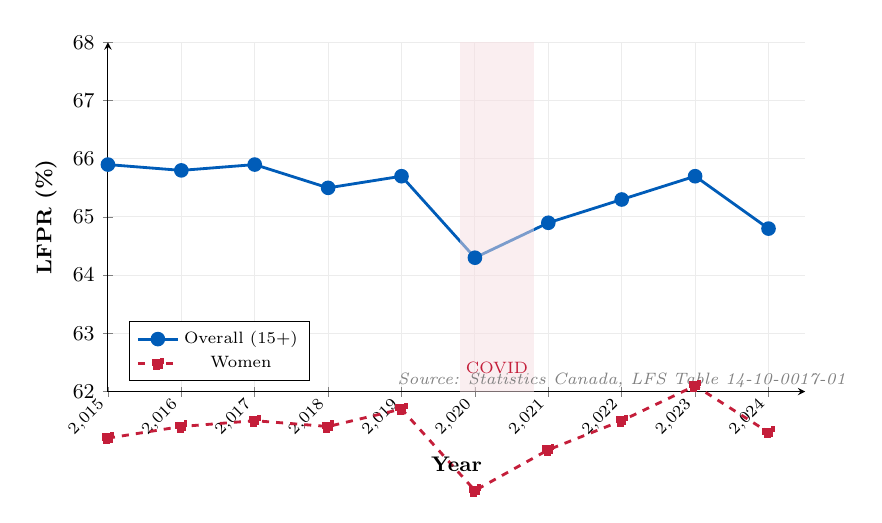
\begin{tikzpicture}[scale=0.85]
  \begin{axis}[
    width=12cm, height=6.8cm,
    xlabel={\textbf{Year}},
    ylabel={\textbf{LFPR (\%)}},
    xmin=2015, xmax=2024.5,
    ymin=62, ymax=68,
    xtick={2015,2016,2017,2018,2019,2020,2021,2022,2023,2024},
    xticklabel style={rotate=45, anchor=east, font=\scriptsize},
    ytick={62,63,64,65,66,67,68},
    tick label style={font=\small},
    label style={font=\small\bfseries},
    axis lines=left,
    grid=major, grid style={gray!15},
    legend pos=south west, legend style={font=\scriptsize},
    clip=false,
  ]
  % Overall LFPR
  \addplot[very thick, color=accent, mark=*, mark size=2.5pt]
    coordinates {
      (2015,65.9)(2016,65.8)(2017,65.9)(2018,65.5)
      (2019,65.7)(2020,64.3)(2021,64.9)(2022,65.3)
      (2023,65.7)(2024,64.8)
    };
  \addlegendentry{Overall (15+)}
  % Women LFPR (approx)
  \addplot[very thick, color=canadared, dashed, mark=square*, mark size=2pt]
    coordinates {
      (2015,61.2)(2016,61.4)(2017,61.5)(2018,61.4)
      (2019,61.7)(2020,60.3)(2021,61.0)(2022,61.5)
      (2023,62.1)(2024,61.3)
    };
  \addlegendentry{Women}
  % COVID annotation
  \fill[canadared!15, opacity=0.5]
    (axis cs:2019.8,62) rectangle (axis cs:2020.8,68);
  \node[font=\scriptsize, text=canadared, align=center]
    at (axis cs:2020.3,62.4) {COVID};
  \node[font=\scriptsize\itshape, text=gray]
    at (axis cs:2022,62.2)
    {Source: Statistics Canada, LFS Table 14-10-0017-01};
  \end{axis}
\end{tikzpicture}
\end{center}
\end{frame}

\begin{frame}{Problems with Measuring Unemployment}
\transfade
\begin{itemize}[<+->]
  \item The measured UR is \textbf{not perfect}.
  \item May \alert{understate} true unemployment:
  \begin{itemize}[<+->]
    \item \textbf{Discouraged workers:} stopped looking but would accept a job --- classified as ``not in the labour force.''
    \item \textbf{Underemployment:} part-time workers who want full-time work; those in jobs below their skill level.
    \item Statistics Canada's \textbf{R8 rate} includes these: in 2024, R8 $\approx$9.8\% vs.\ official UR of 6.3\%.
  \end{itemize}
  \item May \alert{overstate} unemployment:
  \begin{itemize}[<+->]
    \item Some people claim to search while not seriously looking (to retain benefits).
  \end{itemize}
\end{itemize}
\end{frame}

% ============================================================
\section{5.2 Types of Unemployment}
% ============================================================

\begin{frame}{5.2 Learning Objective}
\transfade
\begin{block}{Goal}
Identify and understand the four types of unemployment.
\end{block}
\end{frame}

%--- Fig 5.3: Canadian unemployment rate ---
\begin{frame}{Figure 5.3 -- Canadian Unemployment Rate 2015--2024}
\begin{center}
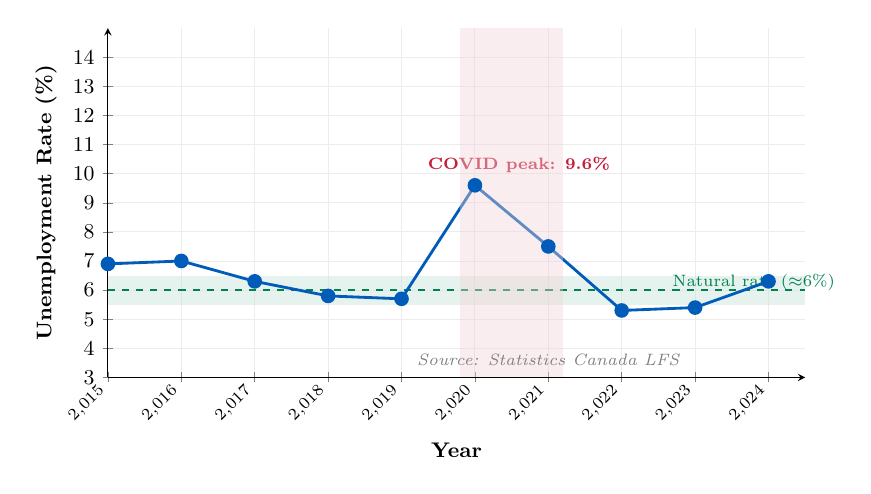
\begin{tikzpicture}[scale=0.85]
  \begin{axis}[
    width=12cm, height=6.8cm,
    xlabel={\textbf{Year}},
    ylabel={\textbf{Unemployment Rate (\%)}},
    xmin=2015, xmax=2024.5,
    ymin=3, ymax=15,
    xtick={2015,2016,2017,2018,2019,2020,2021,2022,2023,2024},
    xticklabel style={rotate=45, anchor=east, font=\scriptsize},
    ytick={3,4,5,6,7,8,9,10,11,12,13,14},
    tick label style={font=\small},
    label style={font=\small\bfseries},
    axis lines=left,
    grid=major, grid style={gray!15},
    clip=false,
  ]
  % Natural rate band (drawn first, behind data line)
  \addplot[fill=leafgreen!20, draw=none, opacity=0.5] coordinates
    {(2015,5.5)(2024.5,5.5)(2024.5,6.5)(2015,6.5)} -- cycle;
  \addplot[thick, color=leafgreen, dashed, domain=2015:2024.5, samples=2] {6.0};
  \node[font=\scriptsize, text=leafgreen]
    at (axis cs:2023.8,6.25) {Natural rate ($\approx$6\%)};
  % Unemployment rate (drawn on top of shading)
  \addplot[very thick, color=accent, mark=*, mark size=2.5pt]
    coordinates {
      (2015,6.9)(2016,7.0)(2017,6.3)(2018,5.8)
      (2019,5.7)(2020,9.6)(2021,7.5)(2022,5.3)
      (2023,5.4)(2024,6.3)
    };
  % COVID peak
  \node[font=\scriptsize\bfseries, text=canadared]
    at (axis cs:2020.6,10.3) {COVID peak: 9.6\%};
  \fill[canadared!20, opacity=0.4]
    (axis cs:2019.8,3) rectangle (axis cs:2021.2,15);
  \node[font=\scriptsize\itshape, text=gray]
    at (axis cs:2021,3.6)
    {Source: Statistics Canada LFS};
  \end{axis}
\end{tikzpicture}
\end{center}
\end{frame}

\begin{frame}{Four Types of Unemployment}
\transfade
\begin{itemize}[<+->]
  \item \textbf{Frictional:} short-term; workers between jobs or entering the market.
  \item \textbf{Structural:} persistent mismatch between worker skills and job requirements.
  \item \textbf{Cyclical:} caused by a recession --- demand for labour falls economy-wide.
  \item \textbf{Seasonal:} due to predictable seasonal patterns (weather, harvest, holidays).
\end{itemize}
\end{frame}

\begin{frame}{Frictional Unemployment}
\transfade
\begin{itemize}[<+->]
  \item \textbf{Frictional unemployment:} short-term unemployment from the process of \textbf{matching} workers to jobs.
  \item Causes:
  \begin{itemize}[<+->]
    \item People entering or re-entering the labour force.
    \item People voluntarily leaving one job to search for a better one.
  \end{itemize}
  \item Some frictional unemployment is \alert{unavoidable} and even \textbf{beneficial}:
  \begin{itemize}[<+->]
    \item better matches $\Rightarrow$ higher productivity.
  \end{itemize}
  \item \textbf{Canadian example:} A recent UBC graduate takes 8 weeks to find an entry-level data analyst role in Vancouver --- this is frictional unemployment.
\end{itemize}
\end{frame}

\begin{frame}{Structural Unemployment}
\transfade
\begin{itemize}[<+->]
  \item \textbf{Structural unemployment:} persistent mismatch between the \textbf{skills} of workers and the \textbf{requirements} of available jobs.
  \item Causes: technological change, industry decline, geographic mismatch.
  \item Tends to be \textbf{longer-term} --- workers may need retraining or relocation.
  \item \textbf{Canadian examples:}
  \begin{itemize}[<+->]
    \item Auto assembly workers in Windsor displaced by automation.
    \item Coal miners in Alberta's Crowsnest Pass as coal demand declines.
    \item Ottawa's Better Jobs program targets retraining for structurally unemployed workers.
  \end{itemize}
\end{itemize}
\end{frame}

\begin{frame}{Cyclical Unemployment}
\transfade
\begin{itemize}[<+->]
  \item \textbf{Cyclical unemployment:} unemployment caused by a \alert{business-cycle recession}.
  \item When aggregate demand falls, firms cut production and lay off workers.
  \item Workers are skilled and would normally be employed --- the problem is insufficient demand.
  \item \textbf{Canadian examples:}
  \begin{itemize}[<+->]
    \item COVID-19 (Spring 2020): unemployment surged from 5.7\% to 13.7\% in two months.
    \item 2008--09 Global Financial Crisis: Canadian UR rose from 6\% to 8.7\%.
    \item Chrysler Brampton Assembly (2009): temporary closure due to low car demand.
  \end{itemize}
\end{itemize}
\end{frame}

\begin{frame}{Seasonal Unemployment}
\transfade
\begin{itemize}[<+->]
  \item \textbf{Seasonal unemployment:} predictable unemployment due to weather, calendar, or demand patterns.
  \item \textbf{Canadian examples:}
  \begin{itemize}[<+->]
    \item Construction workers in Saskatchewan laid off each November.
    \item Ski resort staff in Banff unemployed in summer.
    \item Fish plant workers in N.L. idle between fishing seasons.
    \item Retail staff hired in November--December, let go in January.
  \end{itemize}
  \item Statistics Canada publishes both \textbf{seasonally adjusted} and \textbf{unadjusted} series to separate this effect.
\end{itemize}
\end{frame}

\begin{frame}{Full Employment and the Natural Rate}
\transfade
\begin{itemize}[<+->]
  \item At \textbf{full employment}, all unemployment is frictional and structural --- zero cyclical unemployment.
  \item \textbf{Natural rate of unemployment:} the unemployment rate when the economy is at full employment.
  \[
    u^* = \text{Frictional} + \text{Structural unemployment}
  \]
  \item \textbf{Canadian estimates:} $u^* \approx 5.5$--$6.0\%$ in recent years (Bank of Canada, MPR October 2024).
  \item When actual UR $>$ $u^*$: cyclical unemployment exists $\Rightarrow$ output gap is negative.
\end{itemize}
\end{frame}

% ============================================================
\section{5.3 Explaining Unemployment}
% ============================================================

\begin{frame}{5.3 Learning Objective}
\transfade
\begin{block}{Goal}
Explain what determines the unemployment rate and how policy affects it.
\end{block}
\end{frame}

\begin{frame}{Employment Insurance (EI)}
\transfade
\begin{itemize}[<+->]
  \item \textbf{Employment Insurance (EI):} replaces $\approx$55\% of insurable earnings (max $\approx$\$695/week in 2024).
  \item \textbf{Benefits of EI:}
  \begin{itemize}[<+->]
    \item Gives workers time to find better-matched jobs.
    \item Stabilizes consumer spending during recessions.
  \end{itemize}
  \item \textbf{Costs of EI:}
  \begin{itemize}[<+->]
    \item Reduces the urgency to find work $\Rightarrow$ \textbf{longer average duration} of unemployment.
    \item Estimates suggest EI increases frictional unemployment slightly.
  \end{itemize}
\end{itemize}
\end{frame}

\begin{frame}{Minimum Wage Laws}
\transfade
\begin{itemize}[<+->]
  \item Minimum wages raise the cost of hiring labour for firms.
  \item May cause firms to hire fewer workers, substitute capital for labour, or reduce hours.
\end{itemize}
\vspace{0.3em}
\begin{center}
\renewcommand{\arraystretch}{1.3}
\small
\begin{tabular}{lc}
\toprule
\textbf{Province / Territory} & \textbf{Min.\ Wage (2025)} \\
\midrule
Nunavut & \$19.00/hr \\
British Columbia & \$17.40/hr \\
Ontario & \$17.20/hr \\
Alberta & \$15.00/hr \\
New Brunswick & \$15.30/hr \\
\bottomrule
\end{tabular}
\end{center}
\begin{itemize}[<+->]
  \item Research suggests a 10\% increase in minimum wage reduces teenage employment by $\approx$2\%.
  \item Overall effect on total unemployment is believed to be \textbf{relatively small} (Bank of Canada, 2023).
\end{itemize}
\end{frame}

\begin{frame}{Labour Unions and Efficiency Wages}
\transfade
\begin{itemize}[<+->]
  \item \textbf{Labour unions:} $\approx$30\% of Canadian workers are unionized (2023); $\approx$77\% of public sector vs.\ $\approx$15\% private sector.
  \begin{itemize}[<+->]
    \item Unions push wages above competitive levels for members $\Rightarrow$ some unemployment for non-members.
    \item Limited impact on \textbf{overall} unemployment in Canada.
  \end{itemize}
  \item \textbf{Efficiency wages:} firms voluntarily pay above-market wages to:
  \begin{itemize}[<+->]
    \item reduce turnover (e.g., large banks, tech firms),
    \item increase effort and attract higher-quality workers.
  \end{itemize}
  \item Result: persistent unemployment even in good times --- some workers \emph{want} jobs at the efficiency wage but cannot find them.
\end{itemize}
\end{frame}

% ============================================================
\section{5.4 Measuring Inflation}
% ============================================================

\begin{frame}{5.4 Learning Objective}
\transfade
\begin{block}{Goal}
Define the price level and inflation rate, and understand how they are computed.
\end{block}
\begin{itemize}[<+->]
  \item \textbf{Price level:} average prices of goods and services in the economy.
  \item \textbf{Inflation rate:} percentage increase in the price level from one year to the next.
  \[
    \pi_t = \frac{P_t - P_{t-1}}{P_{t-1}} \times 100
  \]
  \item Key measures: \textbf{CPI}, \textbf{PPI}, and \textbf{GDP deflator}.
\end{itemize}
\end{frame}

%--- Fig 5.4: CPI basket pie chart ---
\begin{frame}{Figure 5.4 -- The Canadian CPI Basket (2023 Weights)}
\begin{center}
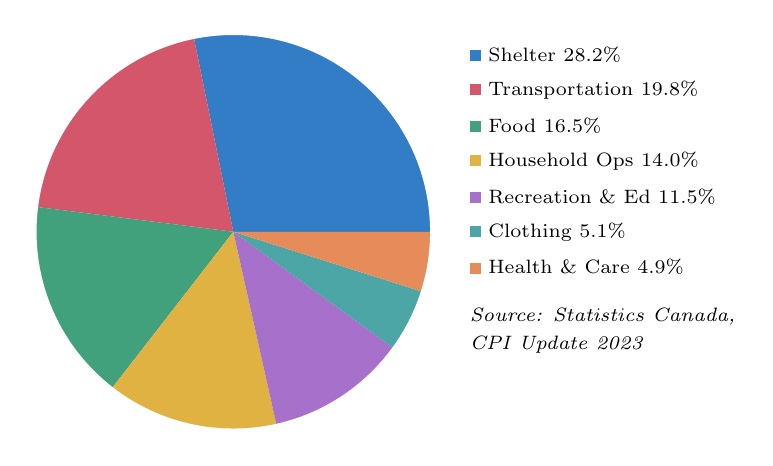
\begin{tikzpicture}[scale=0.9]
  % Pie chart with 7 slices
  % Weights: Shelter 28.2, Transport 19.8, Food 16.5, HH ops 14.0, Rec/Ed 11.5, Health 4.9, Clothing 5.1
  % Using TikZ manual pie slices
  % Total = 100, angles: shelter=101.5, transport=71.3, food=59.4, HH=50.4, Rec=41.4, Health=17.6, Clothing=18.4
  \def\radius{2.8cm}
  % Slice: Shelter (0 -> 101.5 deg)
  \fill[accent!80] (0,0) -- ({cos(0)*\radius},{sin(0)*\radius})
    arc[start angle=0, end angle=101.5, radius=\radius] -- cycle;
  % Slice: Transport (101.5 -> 172.8)
  \fill[canadared!75] (0,0) -- ({cos(101.5)*\radius},{sin(101.5)*\radius})
    arc[start angle=101.5, end angle=172.8, radius=\radius] -- cycle;
  % Slice: Food (172.8 -> 232.2)
  \fill[leafgreen!75] (0,0) -- ({cos(172.8)*\radius},{sin(172.8)*\radius})
    arc[start angle=172.8, end angle=232.2, radius=\radius] -- cycle;
  % Slice: Household operations (232.2 -> 282.6)
  \fill[goldenrod!85] (0,0) -- ({cos(232.2)*\radius},{sin(232.2)*\radius})
    arc[start angle=232.2, end angle=282.6, radius=\radius] -- cycle;
  % Slice: Recreation & Education (282.6 -> 324.0)
  \fill[shiftpurple!70] (0,0) -- ({cos(282.6)*\radius},{sin(282.6)*\radius})
    arc[start angle=282.6, end angle=324.0, radius=\radius] -- cycle;
  % Slice: Clothing (324.0 -> 342.4)
  \fill[tealblue!70] (0,0) -- ({cos(324.0)*\radius},{sin(324.0)*\radius})
    arc[start angle=324.0, end angle=342.4, radius=\radius] -- cycle;
  % Slice: Health & Personal care (342.4 -> 360)
  \fill[deeporange!70] (0,0) -- ({cos(342.4)*\radius},{sin(342.4)*\radius})
    arc[start angle=342.4, end angle=360, radius=\radius] -- cycle;
  % Border
  \draw[white, line width=1.2pt] (0,0) circle (\radius);

  % Legend
  \node[font=\scriptsize, right] at (3.2, 2.5) {\textcolor{accent!80}{\rule{0.5em}{0.5em}}\ Shelter 28.2\%};
  \node[font=\scriptsize, right] at (3.2, 2.0) {\textcolor{canadared!75}{\rule{0.5em}{0.5em}}\ Transportation 19.8\%};
  \node[font=\scriptsize, right] at (3.2, 1.5) {\textcolor{leafgreen!75}{\rule{0.5em}{0.5em}}\ Food 16.5\%};
  \node[font=\scriptsize, right] at (3.2, 1.0) {\textcolor{goldenrod!85}{\rule{0.5em}{0.5em}}\ Household Ops 14.0\%};
  \node[font=\scriptsize, right] at (3.2, 0.5) {\textcolor{shiftpurple!70}{\rule{0.5em}{0.5em}}\ Recreation \& Ed 11.5\%};
  \node[font=\scriptsize, right] at (3.2, 0.0) {\textcolor{tealblue!70}{\rule{0.5em}{0.5em}}\ Clothing 5.1\%};
  \node[font=\scriptsize, right] at (3.2,-0.5) {\textcolor{deeporange!70}{\rule{0.5em}{0.5em}}\ Health \& Care 4.9\%};
  \node[font=\scriptsize\itshape, right] at (3.2,-1.2) {Source: Statistics Canada,};
  \node[font=\scriptsize\itshape, right] at (3.2,-1.6) {CPI Update 2023};
\end{tikzpicture}
\end{center}
\end{frame}

\begin{frame}{The Consumer Price Index (CPI)}
\transfade
\begin{itemize}[<+->]
  \item \textbf{CPI:} measures the average change over time in the prices paid by a typical Canadian household.
  \item Based on a fixed \textbf{basket of goods} (quantities from base period 2002).
  \item \textbf{Formula:}
  \[
    \text{CPI}_t = \frac{\text{Cost of basket in year } t}{\text{Cost of basket in base year}} \times 100
  \]
  \item Used to index wages, pensions, EI benefits, and Old Age Security.
  \item Bank of Canada's inflation target: \textbf{2\%} (with a control range of 1--3\%).
\end{itemize}
\end{frame}

\begin{frame}{Calculating the CPI: A Canadian Example}
\transfade
\small
\begin{itemize}[<+->]
  \item Basket: 5 coffees at Tim Hortons, 1 transit pass, 2 kg of canola oil.
\end{itemize}
\vspace{0.3em}
\renewcommand{\arraystretch}{1.3}
\begin{tabular}{lccccc}
\toprule
 & \multicolumn{2}{c}{\textbf{2002 (base)}} & \multicolumn{2}{c}{\textbf{2024}} & \\
\cmidrule(lr){2-3}\cmidrule(lr){4-5}
\textbf{Item} & Price & Qty & Price & Qty & Note \\
\midrule
Coffee (cup) & \$1.25 & 5 & \$2.50 & 5 & doubled \\
Transit pass & \$60 & 1 & \$105 & 1 & +75\% \\
Canola oil (kg) & \$2.50 & 2 & \$4.00 & 2 & +60\% \\
\midrule
\textbf{Basket cost} & \multicolumn{2}{c}{\$71.25} & \multicolumn{2}{c}{\$128.50} & \\
\bottomrule
\end{tabular}
\begin{itemize}[<+->]
  \item $\text{CPI}_{2024} = \frac{128.50}{71.25} \times 100 \approx \mathbf{180.4}$
  \item This means prices in this basket rose $\approx$80\% since 2002.
\end{itemize}
\end{frame}

%--- Fig 5.5: Canadian CPI inflation rate ---
\begin{frame}{Figure 5.5 -- Canadian CPI Inflation Rate 2015--2024}
\begin{center}
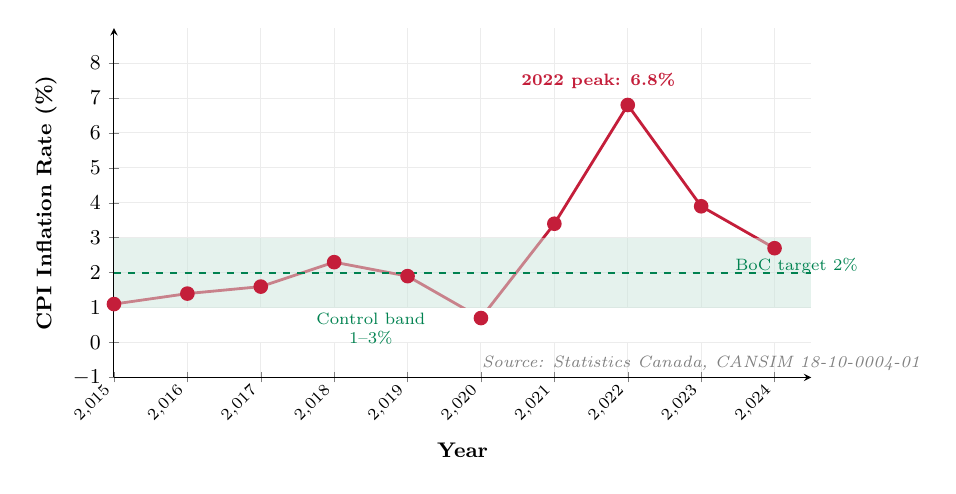
\begin{tikzpicture}[scale=0.85]
  \begin{axis}[
    width=12cm, height=6.8cm,
    xlabel={\textbf{Year}},
    ylabel={\textbf{CPI Inflation Rate (\%)}},
    xmin=2015, xmax=2024.5,
    ymin=-1, ymax=9,
    xtick={2015,2016,2017,2018,2019,2020,2021,2022,2023,2024},
    xticklabel style={rotate=45, anchor=east, font=\scriptsize},
    ytick={-1,0,1,2,3,4,5,6,7,8},
    tick label style={font=\small},
    label style={font=\small\bfseries},
    axis lines=left,
    grid=major, grid style={gray!15},
    clip=false,
  ]
  % CPI inflation (approximate Statistics Canada data)
  \addplot[very thick, color=canadared, mark=*, mark size=2.5pt]
    coordinates {
      (2015,1.1)(2016,1.4)(2017,1.6)(2018,2.3)
      (2019,1.9)(2020,0.7)(2021,3.4)(2022,6.8)
      (2023,3.9)(2024,2.7)
    };
  % Target band
  \addplot[fill=leafgreen!20, opacity=0.5, draw=none, domain=2015:2024.5, samples=2]
    {3} \closedcycle;
  \addplot[fill=white, opacity=1, draw=none, domain=2015:2024.5, samples=2]
    {1} \closedcycle;
  \addplot[thick, color=leafgreen, dashed, domain=2015:2024.5, samples=2] {2};
  \node[font=\scriptsize, text=leafgreen]
    at (axis cs:2024.3,2.2) {BoC target 2\%};
  \node[font=\scriptsize, text=leafgreen, align=center]
    at (axis cs:2018.5,0.4) {Control band\\1--3\%};
  % 2022 peak annotation
  \node[font=\scriptsize\bfseries, text=canadared]
    at (axis cs:2021.6,7.5) {2022 peak: 6.8\%};
  \node[font=\scriptsize\itshape, text=gray]
    at (axis cs:2023,-.6)
    {Source: Statistics Canada, CANSIM 18-10-0004-01};
  \end{axis}
\end{tikzpicture}
\end{center}
\end{frame}

\begin{frame}{Is the CPI Accurate? Four Biases}
\transfade
\begin{itemize}[<+->]
  \item The CPI tends to \alert{overstate} true inflation by $\approx$0.5--1 percentage point per year.
  \item \textbf{Substitution bias:} fixed basket ignores consumers switching to cheaper substitutes.
  \begin{itemize}[<+->]
    \item If beef prices rise, consumers buy more chicken --- but the basket keeps both at old quantities.
  \end{itemize}
  \item \textbf{Quality change bias:} price increases partly reflect better quality (e.g., safer, more fuel-efficient cars).
  \item \textbf{New product bias:} smartphones, streaming services entered the basket with a lag.
  \item \textbf{Outlet bias:} shift to Costco, Amazon, and discount retailers not fully reflected.
\end{itemize}
\end{frame}

\begin{frame}{Producer Price Index (PPI)}
\transfade
\begin{itemize}[<+->]
  \item \textbf{PPI:} measures average prices received by \textbf{producers} at all stages of production.
  \item Basket includes raw materials, semi-finished goods, and wholesale prices.
  \item Changes in the PPI \alert{lead} changes in the CPI:
  \begin{itemize}[<+->]
    \item Higher input costs today $\Rightarrow$ higher retail prices tomorrow.
    \item \textbf{Example:} Surging global wheat prices in 2022 (Russia--Ukraine war) raised PPI for Canadian bakers $\Rightarrow$ grocery bread prices followed within 3--6 months.
  \end{itemize}
\end{itemize}
\end{frame}

% ============================================================
\section{5.5 Using Price Indexes to Adjust for Inflation}
% ============================================================

\begin{frame}{5.5 Learning Objective}
\transfade
\begin{block}{Goal}
Use price indexes to adjust nominal values for inflation.
\end{block}
\begin{itemize}[<+->]
  \item To compare purchasing power across years, convert nominal amounts to \textbf{real} amounts.
  \[
    \text{Real value}_t = \text{Nominal value}_s \times \frac{\text{CPI}_t}{\text{CPI}_s}
  \]
\end{itemize}
\end{frame}

\begin{frame}{Adjusting for Inflation: Canadian Examples}
\transfade
\begin{itemize}[<+->]
  \item \textbf{Example 1 -- Minimum wage:}
  \begin{itemize}[<+->]
    \item Ontario minimum wage was \$10.25/hr in 2014; CPI was 122. In 2024, CPI $\approx$165.
    \[
      \text{Real}_{2024} = 10.25 \times \frac{165}{122} \approx \$13.86/\text{hr}
    \]
    \item Ontario's actual 2024 minimum of \$17.20/hr represents a genuine real increase.
  \end{itemize}
  \item \textbf{Example 2 -- Average weekly earnings:}
  \begin{itemize}[<+->]
    \item Average weekly earnings 2014: \$953; 2024: \$1,260.
    \item Nominal increase: +32\%. CPI increase 2014--2024: $\approx$35\%.
    \item Real wages actually \textbf{fell} slightly.
  \end{itemize}
\end{itemize}
\end{frame}

% ============================================================
\section{5.6 Real versus Nominal Interest Rates}
% ============================================================

\begin{frame}{5.6 Learning Objective}
\transfade
\begin{block}{Goal}
Distinguish between nominal and real interest rates.
\end{block}
\begin{itemize}[<+->]
  \item \textbf{Nominal interest rate ($i$):} the stated rate on a loan or deposit.
  \item \textbf{Real interest rate ($r$):} the nominal rate adjusted for inflation:
  \[
    r \approx i - \pi
  \]
  \item The real rate measures the \textbf{true purchasing-power gain} from lending (or cost of borrowing).
\end{itemize}
\end{frame}

%--- Fig 5.6: Bank of Canada policy rate vs inflation ---
\begin{frame}{Figure 5.6 -- Bank of Canada Policy Rate vs.\ CPI Inflation 2019--2024}
\begin{center}
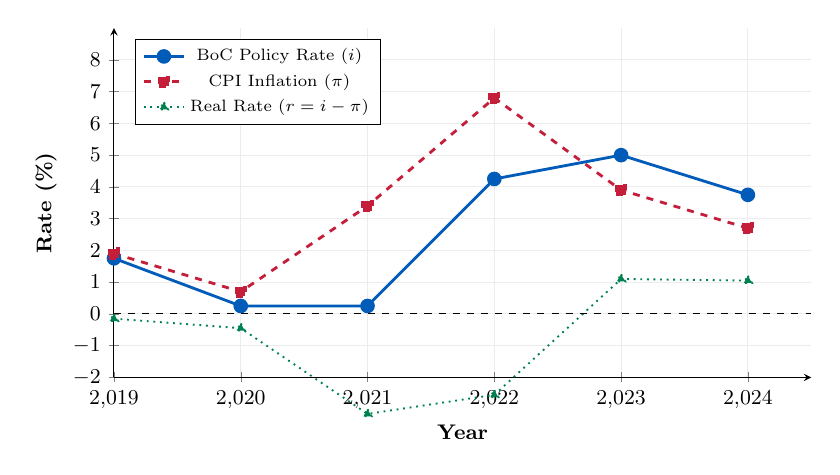
\begin{tikzpicture}[scale=0.85]
  \begin{axis}[
    width=12cm, height=6.8cm,
    xlabel={\textbf{Year}},
    ylabel={\textbf{Rate (\%)}},
    xmin=2019, xmax=2024.5,
    ymin=-2, ymax=9,
    xtick={2019,2020,2021,2022,2023,2024},
    xticklabel style={font=\small},
    ytick={-2,-1,0,1,2,3,4,5,6,7,8},
    tick label style={font=\small},
    label style={font=\small\bfseries},
    axis lines=left,
    grid=major, grid style={gray!15},
    legend pos=north west, legend style={font=\scriptsize},
    clip=false,
  ]
  % Bank of Canada overnight rate (approximate)
  \addplot[very thick, color=accent, mark=*, mark size=2.5pt]
    coordinates {
      (2019,1.75)(2020,0.25)(2021,0.25)(2022,4.25)(2023,5.0)(2024,3.75)
    };
  \addlegendentry{BoC Policy Rate ($i$)}
  % CPI inflation
  \addplot[very thick, color=canadared, dashed, mark=square*, mark size=2pt]
    coordinates {
      (2019,1.9)(2020,0.7)(2021,3.4)(2022,6.8)(2023,3.9)(2024,2.7)
    };
  \addlegendentry{CPI Inflation ($\pi$)}
  % Real rate = i - pi (shaded area)
  \addplot[thick, color=leafgreen, dotted, mark=triangle*, mark size=2pt]
    coordinates {
      (2019,-0.15)(2020,-0.45)(2021,-3.15)(2022,-2.55)(2023,1.1)(2024,1.05)
    };
  \addlegendentry{Real Rate ($r = i - \pi$)}
  \draw[dashed, color=black, thin] (axis cs:2019,0) -- (axis cs:2024.5,0);
  \end{axis}
\end{tikzpicture}
\end{center}
{\scriptsize\itshape Source: Bank of Canada; Statistics Canada CANSIM 18-10-0004-01. Approximate annual averages.}
\end{frame}

\begin{frame}{Real vs.\ Nominal Interest Rates: Canadian Context}
\transfade
\begin{itemize}[<+->]
  \item 2021: BoC policy rate = 0.25\%, inflation = 3.4\% $\Rightarrow$ real rate = \textbf{--3.15\%} --- borrowers were rewarded!
  \item 2023: BoC policy rate = 5.0\%, inflation = 3.9\% $\Rightarrow$ real rate = \textbf{+1.1\%} --- tighter conditions.
  \item 2024: BoC began cutting rates as inflation returned toward 2\%.
  \item \textbf{Key lesson:} a high nominal rate is not necessarily tight if inflation is also high --- what matters for real decisions is the \textbf{real rate}.
\end{itemize}
\end{frame}

% ============================================================
\section{5.7 Does Inflation Impose Costs?}
% ============================================================

\begin{frame}{5.7 Learning Objective}
\transfade
\begin{block}{Goal}
Discuss the problems inflation can cause, even when anticipated.
\end{block}
\end{frame}

\begin{frame}{Is Inflation a Problem?}
\transfade
\begin{itemize}[<+->]
  \item If all prices and wages rose at \textbf{exactly the same rate}: relative prices unchanged, purchasing power unchanged --- inflation would be harmless.
  \item In practice:
  \begin{itemize}[<+->]
    \item Not all prices adjust simultaneously or equally.
    \item Some wages are fixed in long-term contracts.
    \item Cash and fixed-income assets lose real value.
  \end{itemize}
  \item \textbf{Canadian 2022 example:} Grocery prices rose $\approx$10\% while many workers on annual contracts saw only 3--4\% raises --- real wages fell.
\end{itemize}
\end{frame}

\begin{frame}{Costs of Anticipated Inflation}
\transfade
\begin{itemize}[<+->]
  \item \textbf{Redistribution of income:} workers on fixed contracts lose purchasing power; asset owners with real assets (houses, stocks) gain.
  \item \textbf{Loss of purchasing power of cash:} ``shoe-leather costs'' --- people make more trips to the bank, hold less cash.
  \item \textbf{Menu costs:} firms must update price lists, menus, vending machines --- real resource costs. Canada's restaurant sector spent heavily reprinting menus in 2022.
  \item \textbf{Bracket creep:} nominal income rises with inflation, pushing households into higher tax brackets even if real income is unchanged.
  \item \textbf{Taxation of nominal returns:} investors taxed on nominal capital gains even when the real return is zero.
\end{itemize}
\end{frame}

\begin{frame}{Costs of Unanticipated Inflation}
\transfade
\begin{itemize}[<+->]
  \item \textbf{Unanticipated inflation} is especially harmful --- it makes long-term contracting difficult.
  \item \textbf{Borrowers vs.\ lenders:}
  \begin{itemize}[<+->]
    \item Higher-than-expected inflation: borrowers \textbf{gain} (repay in cheaper dollars); lenders \textbf{lose}.
    \item Lower-than-expected inflation: borrowers \textbf{lose}; lenders \textbf{gain}.
  \end{itemize}
  \item \textbf{Canadian 1980s example:} Mortgage rates reached 18--21\%; homeowners who locked in suffered when inflation and rates fell later.
  \item \textbf{2021--22 example:} Many fixed-rate mortgage holders are now renewing at rates 3--4$\times$ higher --- an unanticipated real cost.
  \item Unpredictable inflation discourages saving, investment, and long-term planning.
\end{itemize}
\end{frame}

% ============================================================
\section*{Chapter Summary}
% ============================================================

\begin{frame}{Things to Remember}
\transfade
\begin{itemize}[<+->]
  \item The unemployment rate, LFPR, and ER together describe labour market health --- no single number tells the whole story.
  \item Four types of unemployment: frictional (unavoidable), structural (skill mismatch), cyclical (recession), seasonal (weather/calendar).
  \item CPI measures cost of living; it has biases that cause it to \alert{overstate} inflation by $\approx$0.5--1\%.
  \item Real values = nominal values adjusted by a price index --- always use real for welfare comparisons.
  \item Real interest rate $\approx$ nominal rate $-$ inflation rate --- what matters for borrowing and saving decisions.
  \item Inflation, especially unanticipated, redistributes income and distorts economic decisions.
\end{itemize}
\end{frame}

\begin{frame}{Chapter Summary}
\transfade
\begin{itemize}[<+->]
  \item Statistics Canada measures labour market via LFS ($\approx$56,000 households/month).
  \item Natural rate $u^* \approx 5.5$--$6\%$; cyclical UR in 2020 peaked at 13.7\% (COVID).
  \item Bank of Canada targets 2\% CPI inflation; in 2022 CPI hit 6.8\% --- highest since 1982.
  \item CPI basket: shelter (28\%), transport (20\%), food (17\%) are the largest components.
  \item Real interest rate in 2021: $\approx$ --3\%; in 2023: $\approx$ +1\% --- dramatic shift in monetary conditions.
  \item Unanticipated inflation creates winners (borrowers) and losers (lenders, fixed-income holders).
\end{itemize}
\end{frame}

\begin{frame}
\centering
\Huge \textbf{Thank you!}\\[1em]
\normalsize Questions?\\[0.5em]
\small\itshape Data: Statistics Canada LFS (14-10-0017-01), CPI (18-10-0004-01), National Accounts; Bank of Canada MPR 2024
\end{frame}

\end{document}
